\subsubsection{Giao diện Admin - Quản lý hồ sơ ứng tuyển}

\begin{itemize}
    \item \textbf{Query with composite condition}: Để fetch lên dữ liệu toàn bộ hồ sơ ứng tuyển trong hệ thống theo cơ chế phân trang
    \begin{figure}[H]
        \centering
        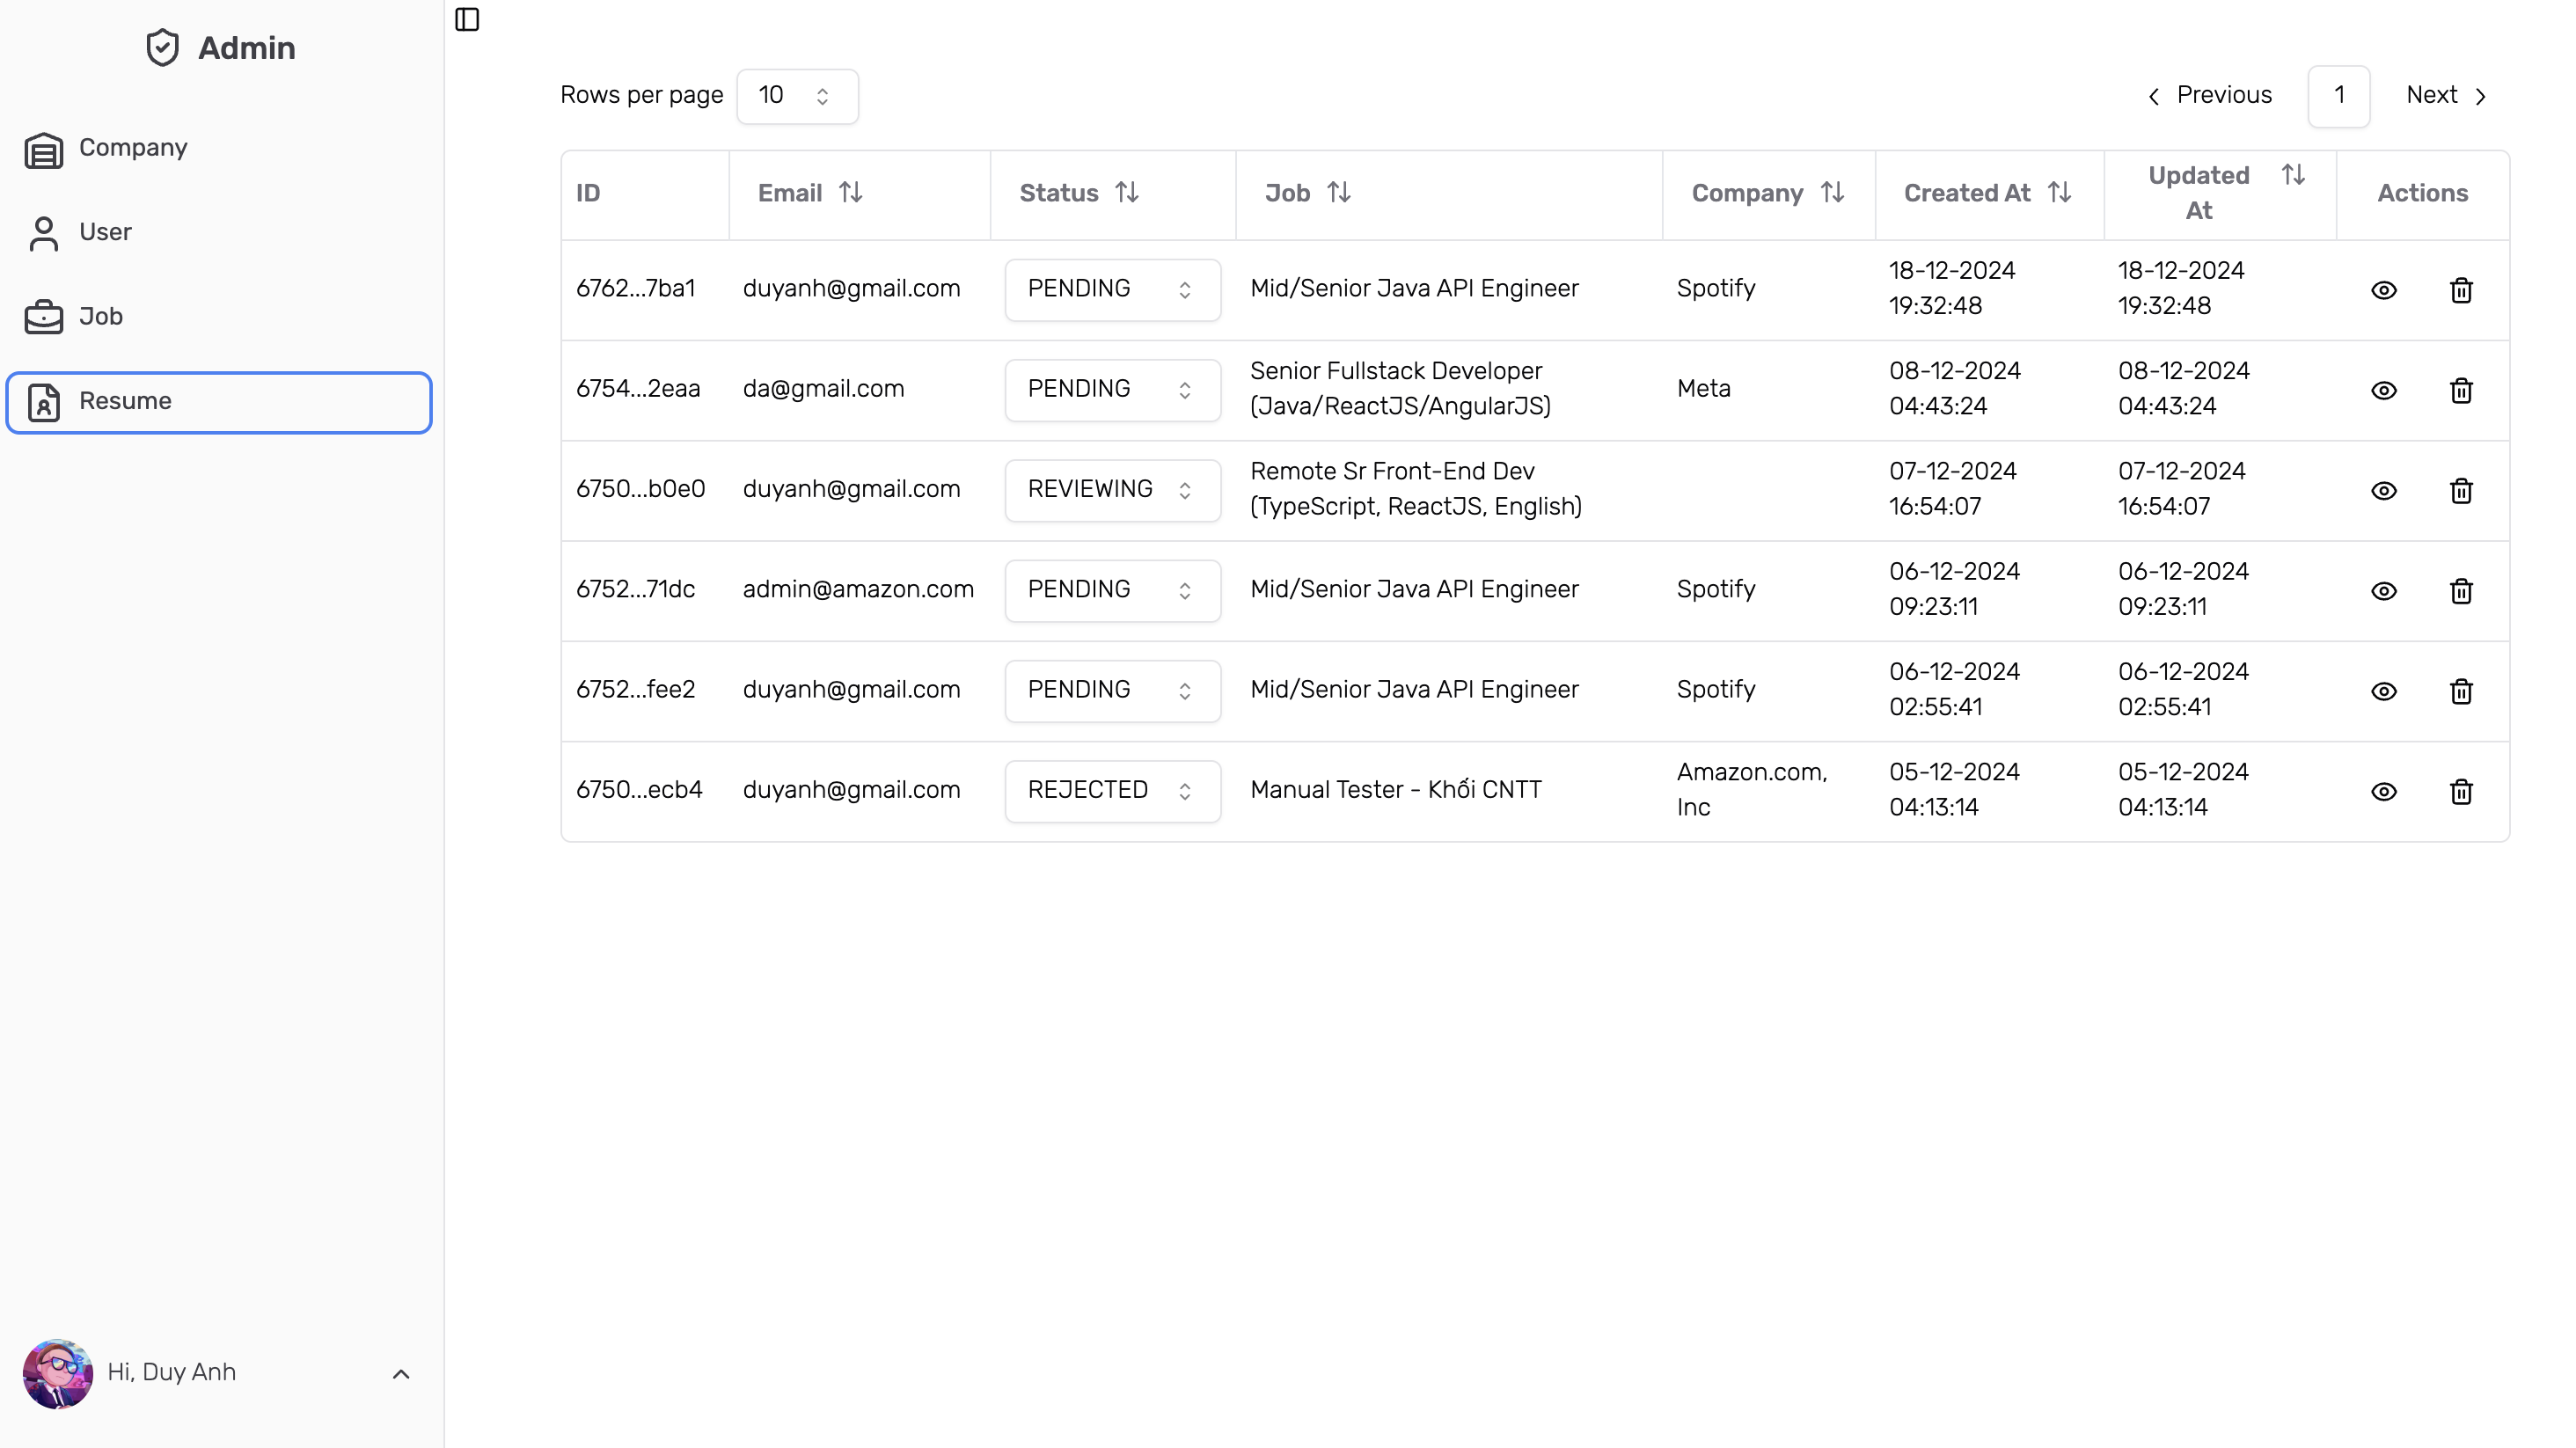
\includegraphics[width=\linewidth]{DBMS-Application/Images/admin-resume.png}
        \caption{Trang quản lý hồ sơ ứng tuyển - Danh sách hồ sơ ứng tuyển trong hệ thống}
        \label{fig:enter-label}
    \end{figure}

    \item \textbf{Update}: Cập nhật thông tin của hồ sơ ứng tuyển, cụ thể là cập nhật \textbf{trạng thái}
    \begin{figure}[H]
        \centering
        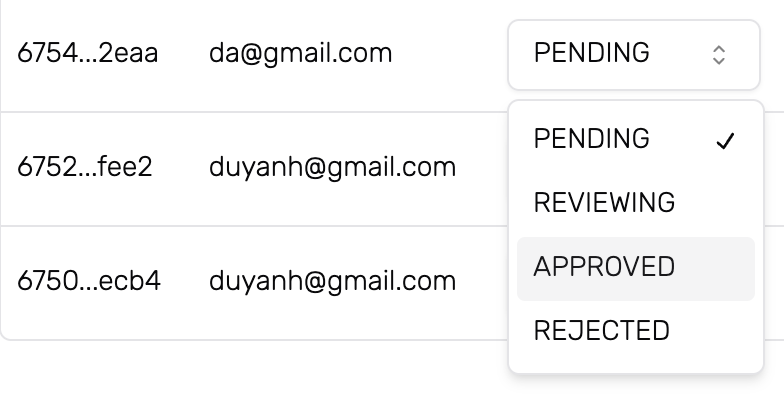
\includegraphics[width=.5\linewidth]{DBMS-Application/Images/update-status-resume.png}
        \caption{Trang quản lý hồ sơ ứng tuyển - Chọn trạng thái mới cho hồ sơ}
        \label{fig:enter-label}
    \end{figure}

    \begin{figure}[H]
        \centering
        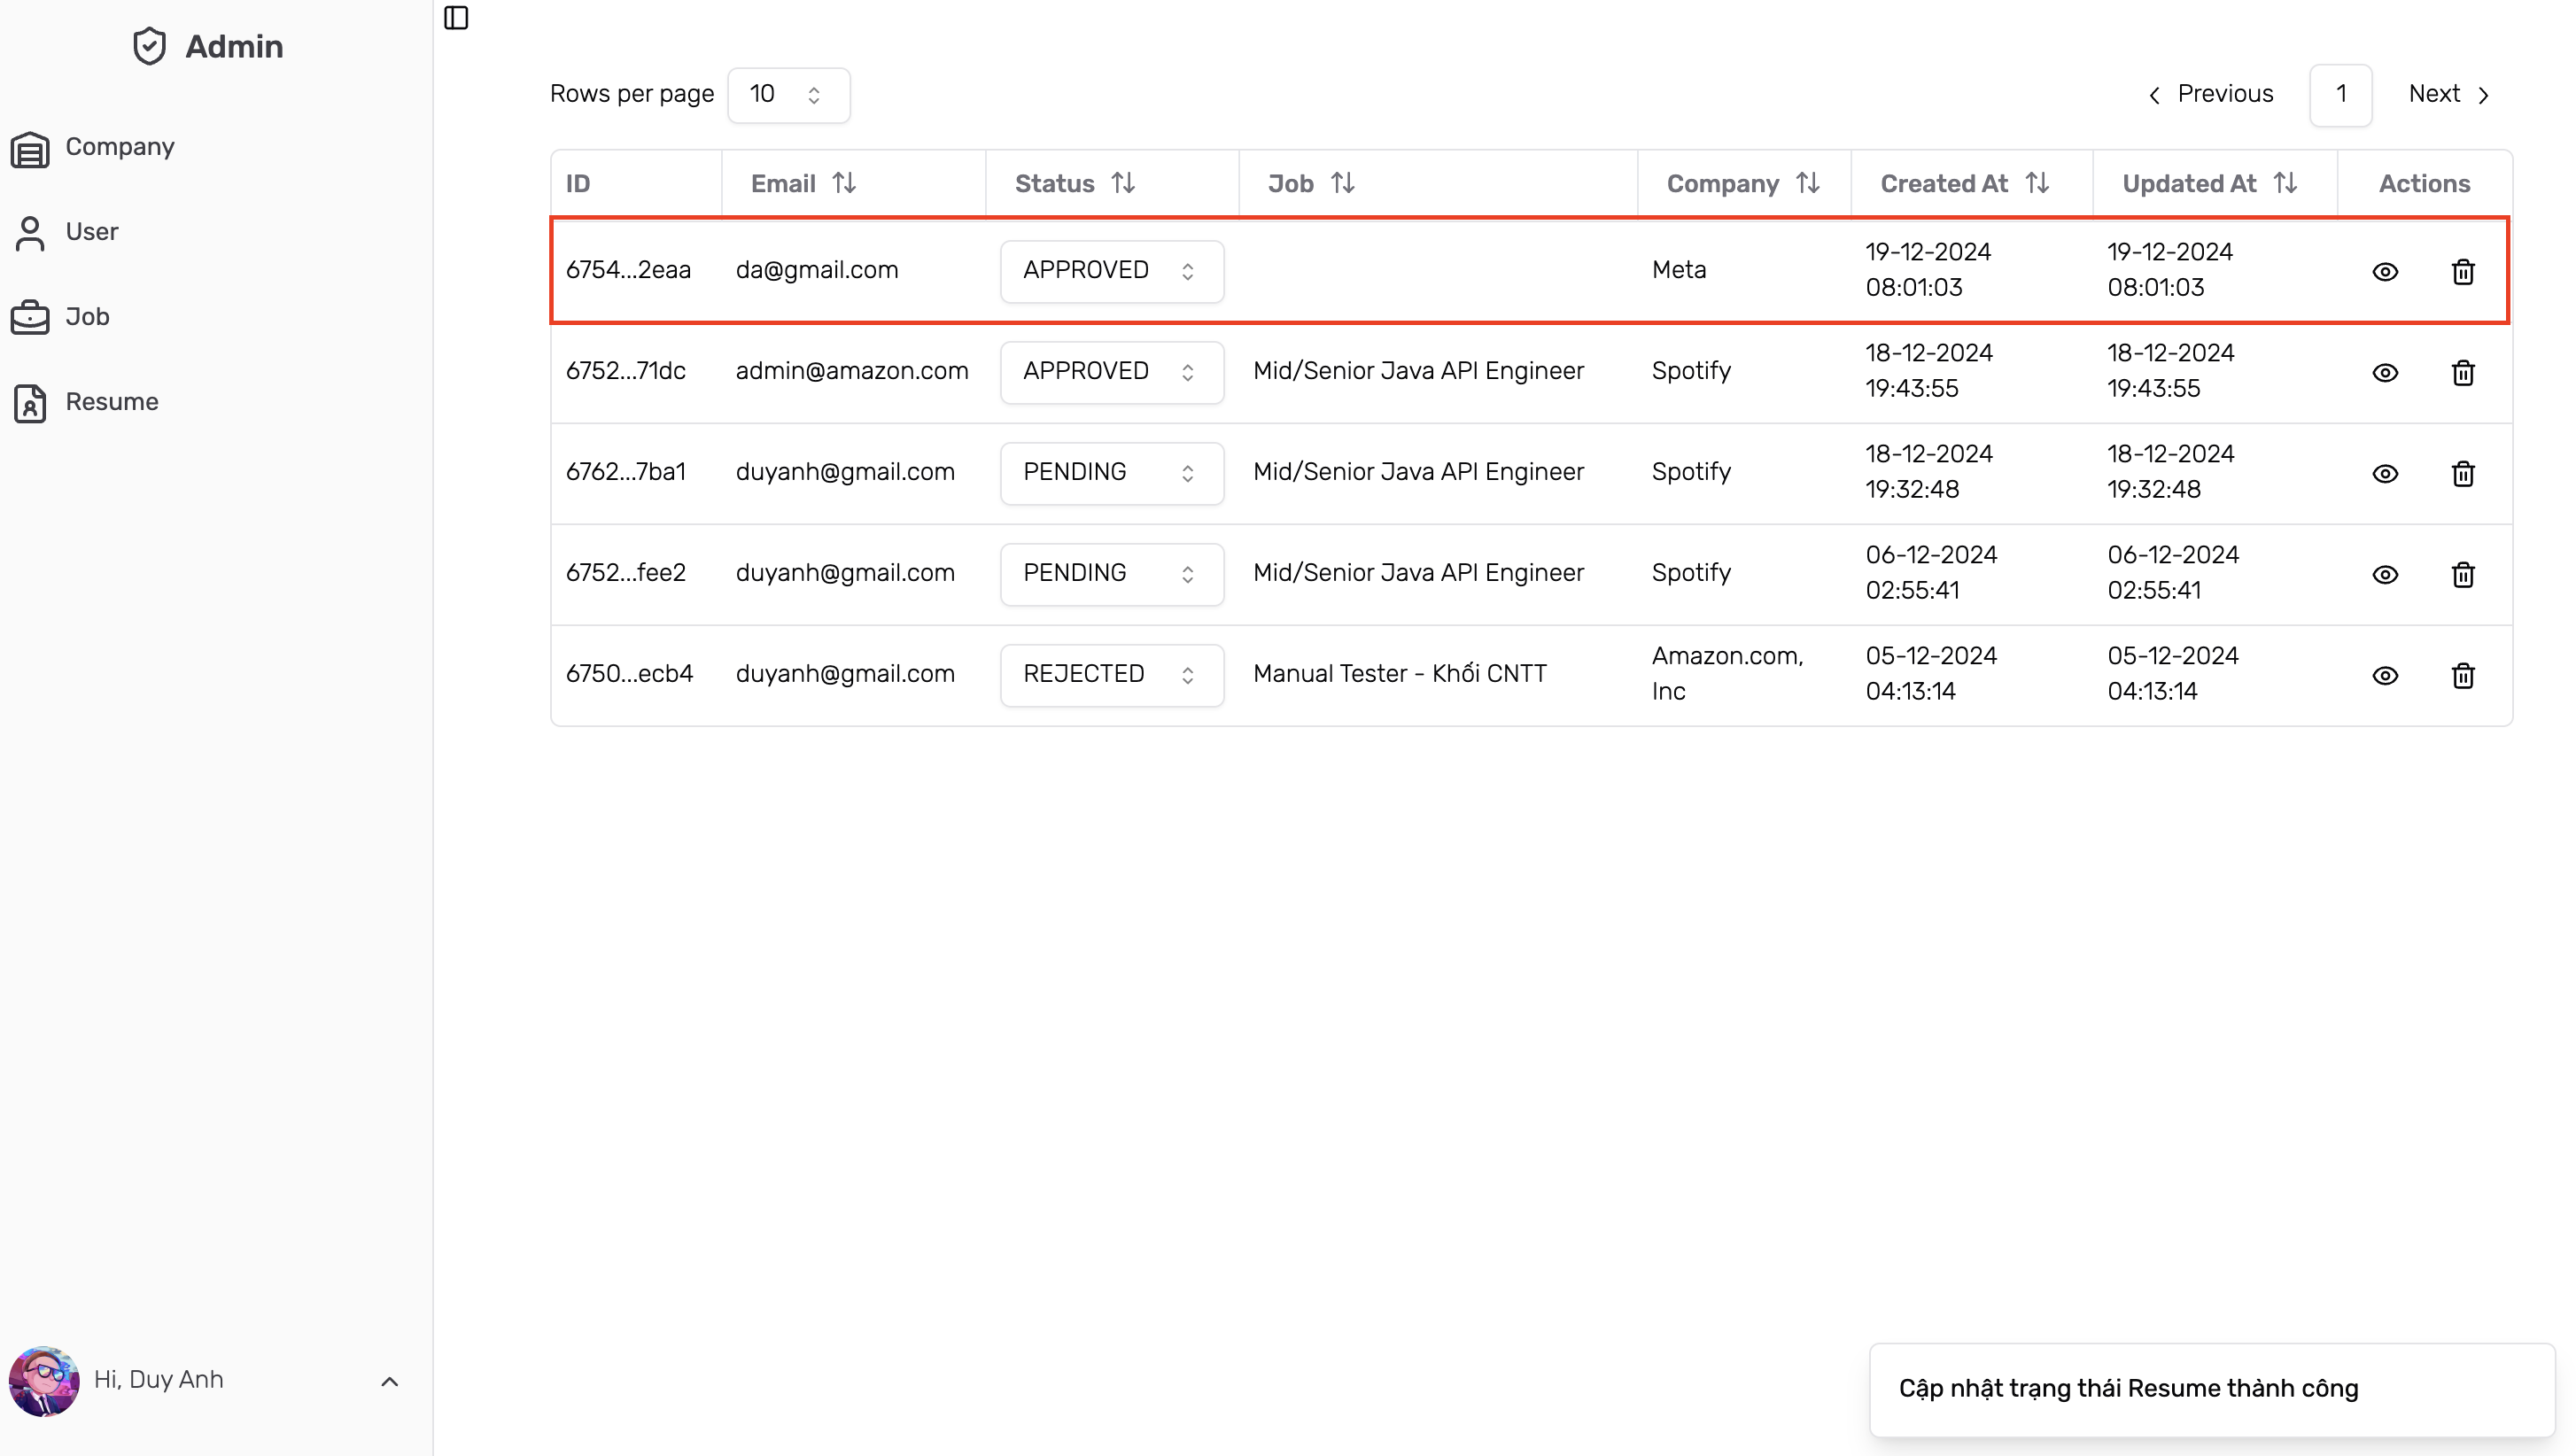
\includegraphics[width=\linewidth]{DBMS-Application/Images/update-resume-successfully.png}
        \caption{Trang quản lý hồ sơ ứng tuyển - Cập nhật trạng thái của hồ sơ ứng tuyển thành công}
        \label{fig:enter-label}
    \end{figure}
    
    \item \textbf{Delete}: Xoá hồ sơ ứng tuyển chỉ định
    \begin{figure}[H]
        \centering
        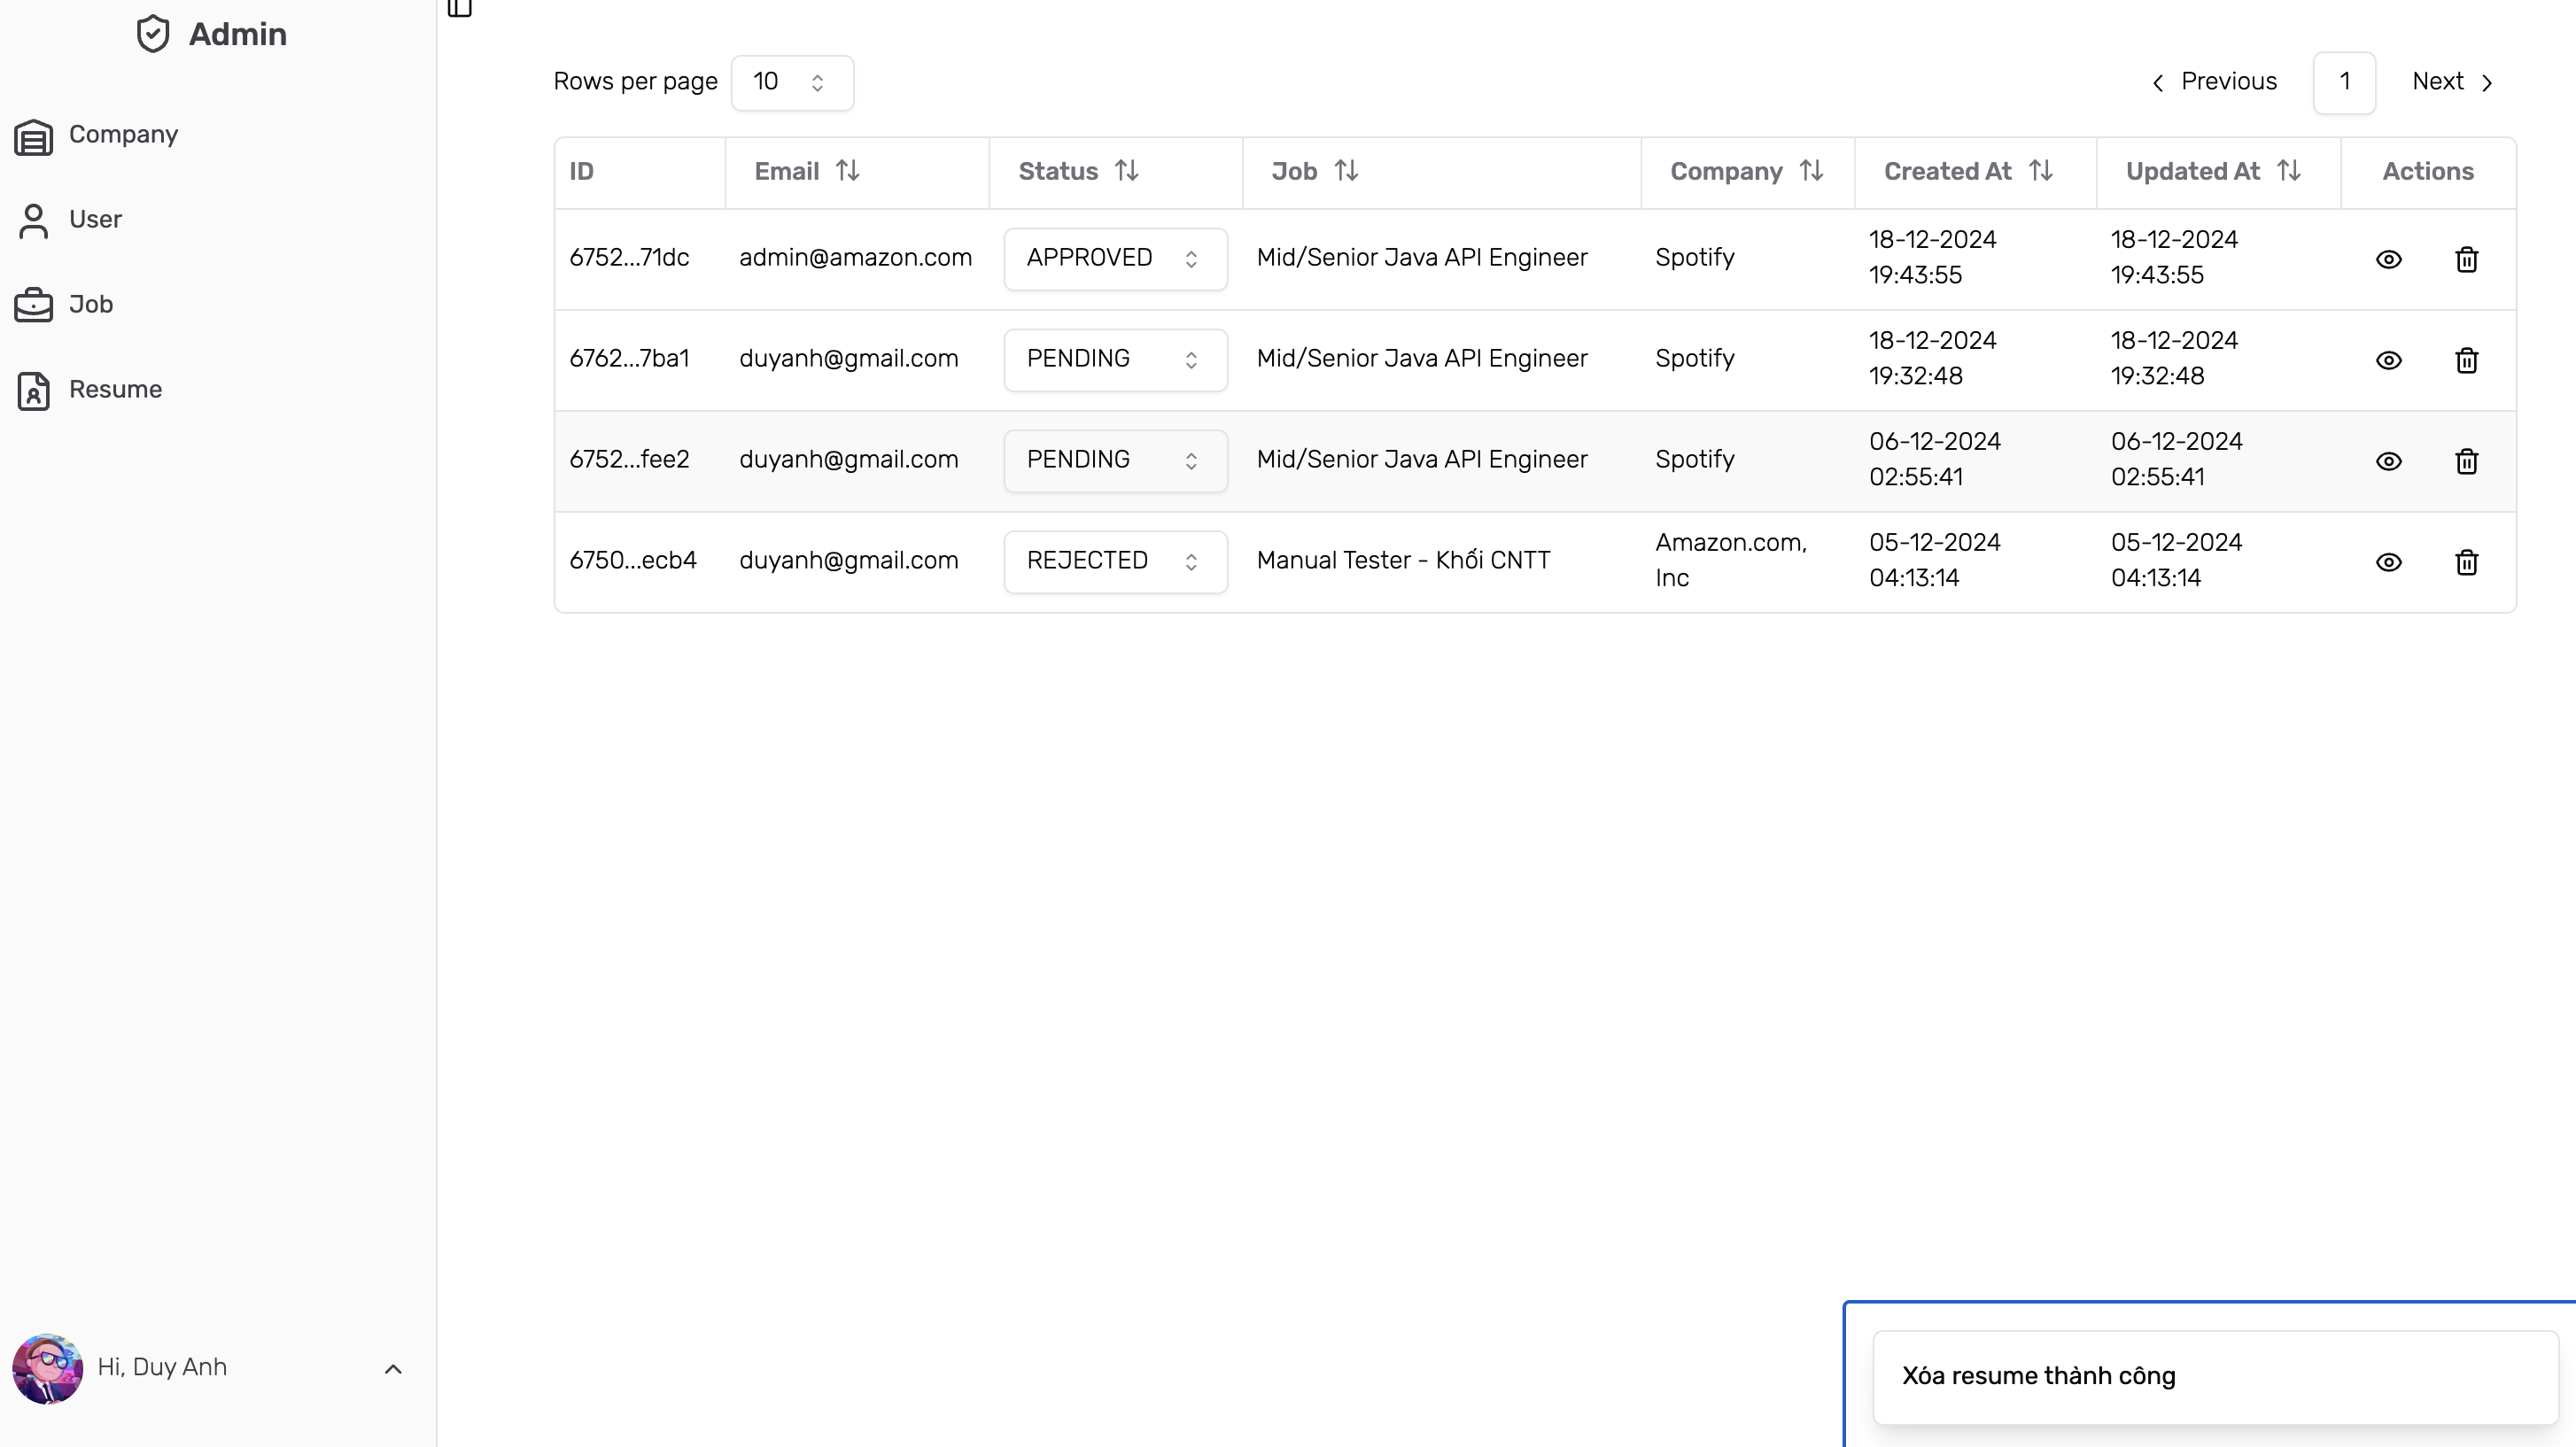
\includegraphics[width=\linewidth]{DBMS-Application/Images/delete-resume.png}
        \caption{Trang quản lý hồ sơ ứng tuyển - Xoá hồ sơ ứng tuyển}
        \label{fig:enter-label}
    \end{figure}
\end{itemize}